\documentclass[journal]{IEEEtran}
\usepackage{graphicx}
\usepackage{float} 
\usepackage{subfigure}

\graphicspath{{figures/}}

\begin{document}

\title{Benchmark Report for MySQL and RocksDB}

\author{Chenxi Huang}

\maketitle

\begin{abstract}
In an era where everyone online is producing data, infrastructures to contain and secure massive data are crucial to all data-related tasks. Database software plays a key role in processing data workload, then higher performance database is beneficial to the efficiency of the whole system. Therefore, measuring the performance of database software is inevitable. In this report, I have run Yahoo! Cloud Serving Benchmark(YCSB) on MySQL \& RocksDB and analyzed the performance data.
\end{abstract}

\begin{IEEEkeywords}
Benchmark, YCSB, MySQL, RocksDB
\end{IEEEkeywords}

\IEEEpeerreviewmaketitle

\section{Introduction}

\IEEEPARstart{T}{o} acquire a picture of the performance of different database software is essential for developers who try to build heavily data-dependent applications. In this sense, doing benchmarks on database software is a necessary approach to gain knowledge of the performance of database software. In this report, I have run a benchmark on database software and made analysis about the performance data revealed from the benchmark.

\section{Benchmark Specification}

\subsection{System Specification}

The benchmark was performed on Ubuntu 22.04. Machine specification is as below:

\begin{itemize}
\item CPU: Intel Core i7 6700k (4 cores, hyperthreading enabled)
\item Memory: DDR4 2133MHz 24 Gigabytes
\item SSD: Intel 600p 512G
\item Linux Kernel Version: 5.15.0-41-generic
\end{itemize}

\subsection{Database Software}

MySQL and RocksDB have been tested in this benchmark. MySQL is an open-source relational database management system(RDBMS), widely used in driving varieties of web applications, initially released in 1995. RocksDB is an embeddable persistant key-value store for fast storage. The RocksDB library is maintained by the Facebook Database Engineering Team, and is based on LevelDB, by Sanjay Ghemawat and Jeff Dean at Google.\cite{ref1} The project maintainers claim that RocksDB excels when running on SSD/RAM. In this benchmark, we used following versions of database software:

\begin{itemize}
\item MySQL 8.0.30
\item RocksDB 7.4.4 (RocksJava, pre-built binary from maven)
\end{itemize}

\subsection{Benchmark Software}

Yahoo! Cloud Serving Benchmark(YCSB) was used in this test. I built JDBC and RocksDB modules of YCSB software from the latest source code(ce3eb9c, 0.18.0-SNAPSHOT).

\subsection{Workloads}

In this benchmark, YCSB offers six core workloads.\cite{ref2}

\subsubsection{Workload A Update heavy workload}

This workload has a mix of 50/50 reads and writes. An application example is a session store recording recent actions. Updates in this workload do not presume you read the original record first. The assumption is all update writes contain fields for a record that already exists; oftentimes writing only a subset of the total fields for that record. Some data stores need to read the underlying record in order to reconcile what the final record should look like, but not all do.

\subsubsection{Workload B Read mostly workload}

This workload has a 95/5 reads/write mix. Application example: photo tagging; add a tag is an update, but most operations are to read tags. As with Workload A, these writes do not presume you read the original record before writing to it.

\subsubsection{Workload C Read only}


This workload is 100\% read. Application example: user profile cache, where profiles are constructed elsewhere (e.g., Hadoop).


\subsubsection{Workload D Read latest workload}


In this workload, new records are inserted, and the most recently inserted records are the most popular. Application example: user status updates; people want to read the latest.


\subsubsection{Workload E Short ranges}


In this workload, short ranges of records are queried, instead of individual records. Application example: threaded conversations, where each scan is for the posts in a given thread (assumed to be clustered by thread id).

\subsubsection{Workload F Read-modify-write}

In this workload, the client will read a record, modify it, and write back the changes. Application example: user database, where user records are read and modified by the user or to record user activity. This workload forces a read of the record from the underlying datastore prior to writing an updated set of fields for that record. This effectively forces all datastores to read the underlying record prior to accepting a write for it. At the moment we use a random delta for the write rather than some value derived from the current record (say incrementing a counter). That can make the workload a bit harder to follow since the starting read seems unnecessary.

\section{Experiment}

\subsection{Measure Approach}

According to the recommended way of doing benchmark by YCSB \cite{ref2}, I loaded workload A's parameter file, and run workload A, B, C, F, D respectively, then reset the database, and load workload E's parameter file and run workload E. Every benchmark was run for 3 times, and throughput data was averaged. Performance was measured for different number of threads used in benchmark queries. The benchmark results were saved to the local disk.

For MySQL, I used YCSB JDBC module to connect MySQL Server with MySQL J Connector under recommended configuration\cite{ref3}. For RocksDB, I adopted pre-built RocksJava binary file to run the benchmark on SSD.

\subsection{Throughput For Each Workload}

\begin{figure}[H]
\centering
\subfigure[Workload A]{
\label{throughput.a}
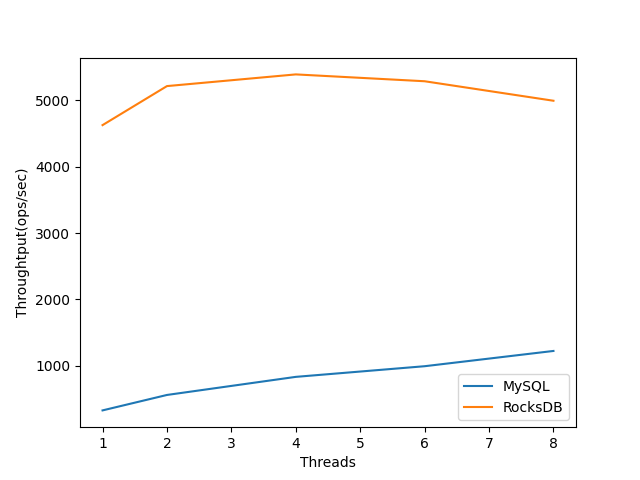
\includegraphics[width=0.22\textwidth]{workload-a}}
\subfigure[Workload B]{
\label{throughput.b}
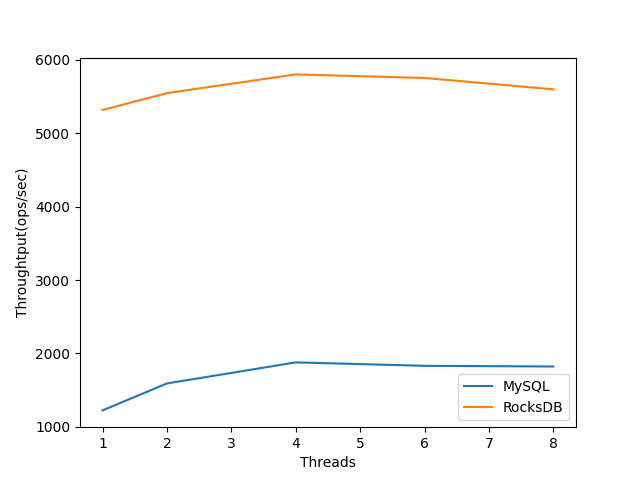
\includegraphics[width=0.22\textwidth]{workload-b}}
\subfigure[Workload C]{
\label{throughput.c}
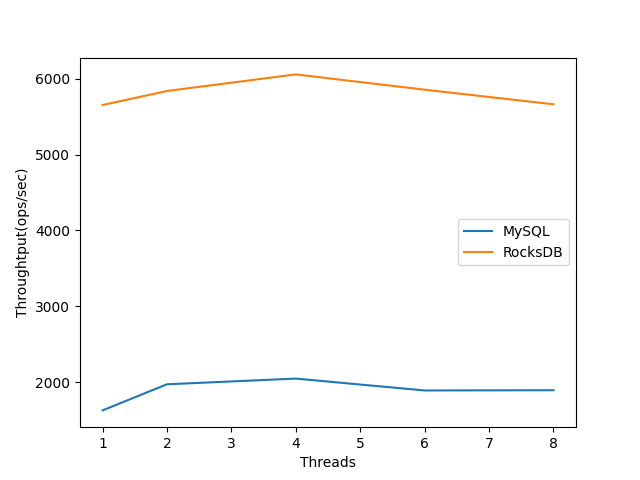
\includegraphics[width=0.22\textwidth]{workload-c}}
\subfigure[Workload D]{
\label{throughput.d}
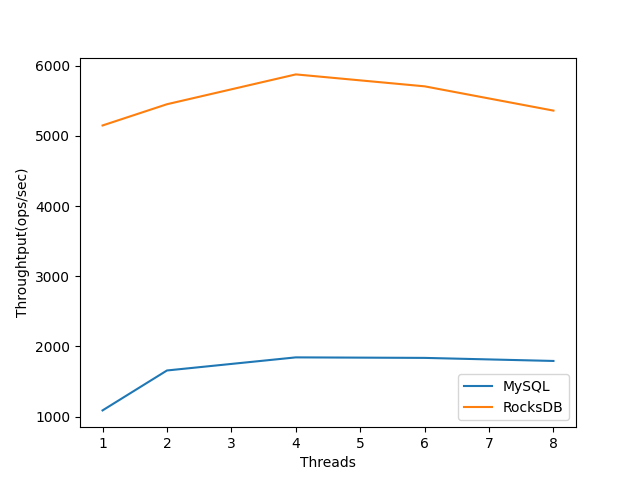
\includegraphics[width=0.22\textwidth]{workload-d}}
\subfigure[Workload E]{
\label{throughput.e}
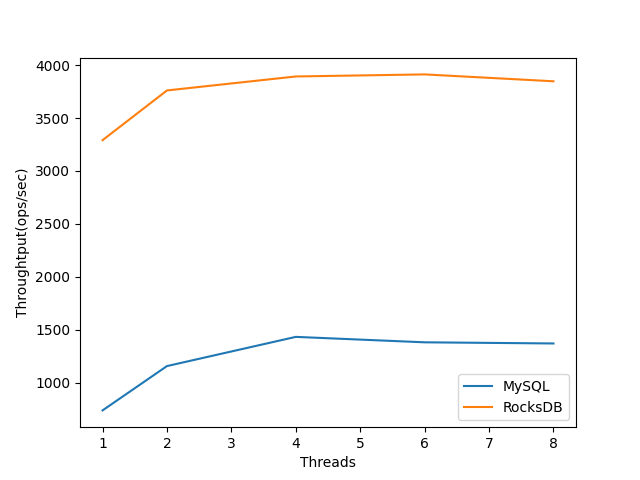
\includegraphics[width=0.22\textwidth]{workload-e}}
\subfigure[Workload F]{
\label{throughput.f}
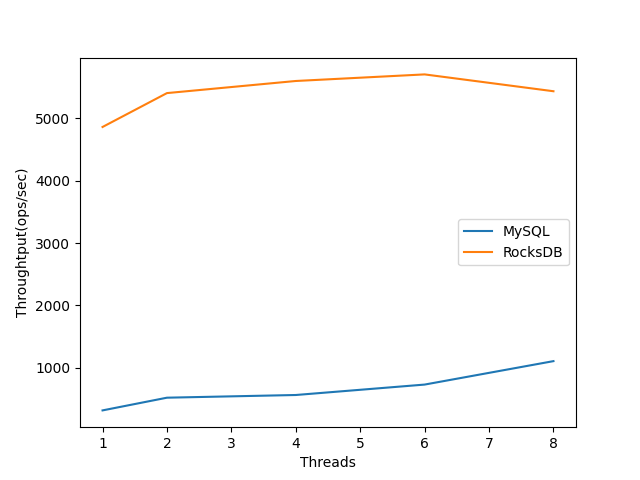
\includegraphics[width=0.22\textwidth]{workload-f}}
\caption{Throughput}
\label{throughput.main}
\end{figure}

\subsection{Facts}

\subsubsection{RocksDB is significantly faster}

The fact that RocksDB is outnumbering MySQL in every workload is clear. In Workload C (Read Only), the read speed of RocksDB is up to 5x faster than MySQL; On the other hand, in Workload A (50/50 reads and writes), the throughput is also 4x to 5x faster.

\subsubsection{Multi-threading performance of RocksDB is unimodal}

For RocksDB throughput in Fig. \ref{throughput.main}, the thread number for optimal performance is around 3 to 6.

\subsubsection{Throughput for MySQL is roughly rising as the thread number adding with exceptions} For Workload A, B, D, E, F, the throughput goes up with slower acceleration. As for read-only Workload C, the throughput is declining.

\subsubsection{The relationship between throughput and thread number} For MySQL, the performance addition is obvious when threads goes from 1 to 2, while the performance growth is not clear when going from 2 to more.

\subsection{Analysis}

\subsubsection{RocksDB takes the advantage of SSD} The higher performance of RocksDB revealed is likely because of its optimization for SSD, while MySQL is developed for general use.

\subsubsection{SQL cost} YCSB operates RocksDB through RocksJava API, while MySQL was connected through local network and operated via SQL queries. I propose that the SQL queries cost is likely responsible for the performance gap.

\subsubsection{Fluctuation of the machine} The machine the benchmark was performed on is powered by Intel Core Series CPU. This series of CPU adjust their clock speed dramatically when heavy load is encountered. I suspect that warm-up time is a possible factor for the performance leap from single thread to dual threads.

\subsection{Possible Improvement}

\subsubsection{Deploying database on more stable machine} It is likely to reduce performance fluctuation when server-class machines with stable clock speed and more cores are equipped, therefore the multi-threaded data point would be collected with more stability and on more cores.

\subsubsection{Doing benchmark on MyRocks} MyRocks is the Facebook version of MySQL, powered by RocksDB as its storage engine. SQL cost and YCSB binding cost can be eliminated from consideration.

\section{Conclusion}

In this benchmark, I have tested MySQL and RocksDB on YCSB test. The test data was collected under YCSB recommended configuration. According to the data, the fact that RocksDB run significantly faster than MySQL is emerged. Other facts are also presented. Then, I propose several points and possible explanations analyzing from the facts. Lastly, I come up with possible improvement for further benchmarking scheme.

\begin{thebibliography}{2}

\bibitem{ref1}RocksDB Official Website - https://rocksdb.org

\bibitem{ref2}Core Workloads - https://github.com/brianfrankcooper/YCSB/wiki/Core-Workloads

\bibitem{ref3}JDBC Driver for YCSB - https://github.com/brianfrankcooper/YCSB/\\ blob/master/jdbc/README.md

\end{thebibliography}

\end{document}


